\chapter{Design Discussion}
\label{ch:design}

\vspace{-1cm}
\begin{center}
Eduard Hirsch
\end{center}

\section{ASIM and blockchain}
\label{sec:asim}

Creating a scalable distributed application is a big challenge. Even more when monolithic legacy systems need to be addressed, like in case of the Sardex payment systems realized on Sardinia. For INTERLACE this meant to deal with a system which is currently stable and working reliably. The drawback of this system is, that it is not scaling well which became more and more evident in recent time and especially will be a problem when provided to multiple other circuits outside of the region besides from the original one in Sardina.

This report will describe a prototypical solution on how distribution and saleability are handled using proper technologies which allow the idea of a mutual credit system to grow and evolve. In detail for INTERLACE an architectural process was introduced which is trying to thoroughly use models that are well tested and shared amongst each other in a very specific and detailed way.

As described in \cite{INTERLACE_D21} an ASM definition has been declared which acts as a ground model for the INTERLACE prototype. Then this paper based definition has been transformed into executable code realized with the ICEF\footnote{Interaction Computing Execution Framework} which is based on ASM language primitives. The next step, which attains main attention in this report, is the last before the actual testing which needs to be done on various levels.

In the following subsections the various topics encountered during planning and evolving of the new blockchain based system are addressed.

\subsection{From Servers to Agents and Peers}

INTERLACE encourages not just a change in technology but also an architectural culture change. Currently many systems in industry are based on monolithic approaches which are stable and based on commonly known and highly adopted implementation strategies.

Often not even based on multiple tiers those classic strategies suit the needs of small and middle sized projects but come at high cost for very large application services and their providers. When increasing in size they become more and more difficult to manage given

\begin{itemize}
	\item their large code base,
	\item non-autonomous teams,
	\item lack in agility,
	\item difficult deployments and
	\item high commitment to specific technologies or even worse vendor lock-ins.
\end{itemize}

Modern large scale architectures therefore aim for finding different possibilities in the field of SOA\footnote{Service Oriented Architecture \cite{erl2014next}} and when advancing further in Micro-Services Architectures. Especially Micro-Services Architectures \cite{newman2015building} claim to solve these problems by providing simple and easy to build applications at the expense of higher network load and more difficult systems integration.

However, INTERLACE, as mentioned before is favouring a different solutions which has similar ideas but is still in most fundamental parts very different, namely, blockchains. Blockchains, like Micro Services, have a highly decentralized distributed nature, regardless, Micro Services deal with an almost purely architectural stile whereas blockchains have a data centric approach and are quite specific in terms of use.

Desirable properties during searching for technologies INTERLACE of blockchains are

\begin{itemize}
	\item Distribution
	\item Peer to Peer communication
	\item Immutable => auditable 
	\item Data storage
	\item Virtual Machine like executions of code (chaincode or Smart Contracts)
\end{itemize}

Further the usage of Smart Contracts or chaincode (Hyperledger Fabric nomenclature) come with various other attributes which are important to manage a mutual credit system. Code executions which are running "on chain" are executed on every peer in the network. In order to be executed correctly chains define roles, state and the code which is attached to a transaction takes care about the business logic and a correct workflow which is writing to the blockchain.

As mentioned before the technology currently use by Sardex lives in a rather monolithic space and it would be extremely difficult and risky to set up a complete distributed blockchain environment and swap systems from one day to another, thus, a road to a complete distributed scenario should be planned keeping in mind that the code base cannot be changed all at once. Speaking of risk means the unclear software and technology requirements but also a possible change of the business model of Sardex as blockchains are quite unique concept with certain implications how users are interacting with the software product.

Consequently, INTERLACE focus has been on understanding the complete core requirements, facilitating the AS(I)M approach, creating a generic model and being independent of technologies used to make the road towards a fully distributed, scalable and reliable system clearer and reduce risks. For INTERLACE this meant further, that the agent based ASIM client-server model has been utilized to create a Hyperledger Composer based implementation.

This Hyperledger Composer business network constructs a blockchain approach which is combining also a Micro Services Architecture. This is not yet a fully distributed scenario but still highly decentralized and also nicely scalable like extending to other circuits or balancing load in-between. In that way it is in addition possible to keep partly control of the blockchain and impose certain rules which otherwise would not yet be clear how to manage them on a completely plain, open-to-the-public blockchain realization.

\subsection{Testing}

This subsection will give a quick overview how testing may be processed for the prototype as well as for the final product. Detailed testing and description of the activities will be reported in D4.1 and D4.2 which will performed after the end of the project.

There are several levels test will take place. As requirements have been defined in ASM language and translated into an ICEF/coreASIM implementation test will take those into account to verify the system. Traditional approaches like the v-model \cite{forsberg1991relationship} usually test on four levels

\begin{itemize}
	\item Acceptance Testing
	\item System Testing
	\item Integration Testing
	\item Unit Testing
\end{itemize}

ASIM models testing can not be put into one of those categories directly. Further, under the umbrella of modern software development methods like (large-scale) scrum, (scaled) agile different testing practices have been adopted.

For D4.1/2 it is planned to test based on the results of the execution of the ASIM Models. Thus, each requirements has a specific output, which is then compared to the log of an execution produced by the new system. This is of course a pretty high level way of testing an may be seen, when comparing to traditional testing, between Integration and System Testing but rather not in the realm of acceptance testing as the requirements defined by ASM are mathematically based algorithms which are difficult to read and to verify by non-technical people.

Due to time-related issues a replacement tool for the ASM comparison test will be used which is called Cucumber\footnote{\url{https://cucumber.io}}. It a scenario based testing tool which combines functional requirements into high level system test which are described as text as well as with domain specific language in order to execute the test. A testing scenario may look like shown in listing \ref{lst:cucumber}.

\begin{center}
\begin{minipage}{0.8\textwidth}
\small
\begin{lstlisting}[language=cucumber,firstnumber=1,caption={\bf\small Cucumber test example},captionpos=b,label=lst:cucumber]
Feature: Perform Credit operations
  Move money from an account of member A to an account of member B
  
  Scenario: account B receives 100 Sardex of account A
    Given: Account A has a positive balance
      And: Account B is able to receive money
      And: Account A has a balance of 100
      And: Account B has a balance of 0
     When: Credit Transaction has performed successfully
     Then: account A has a balance of 0
      And: account B has a balance of 100
\end{lstlisting}
\end{minipage}
\end{center}

The various steps $Given$ [initial context], $When$ [event occurs], $Then$ [ensure some outcomes] are based on a special language called Gherkin\footnote{\url{https://docs.cucumber.io/gherkin}}and elements of it can be connected to test implementations serving that scenario. Details can be looked up at Cucumber Documentation which is publicly available and referenced in the text above.
  
\section{Solution Technologies}
\label{sec:solution}

This last introductory part finally presents the planned solution stack which will be applied for the prototypical solution and is illustrated in figure \ref{fig:solution-stack}. Details on how those components are working together are explained in depth in section \ref{ch:prototype}.

\begin{figure}[htbp]
  \centering
  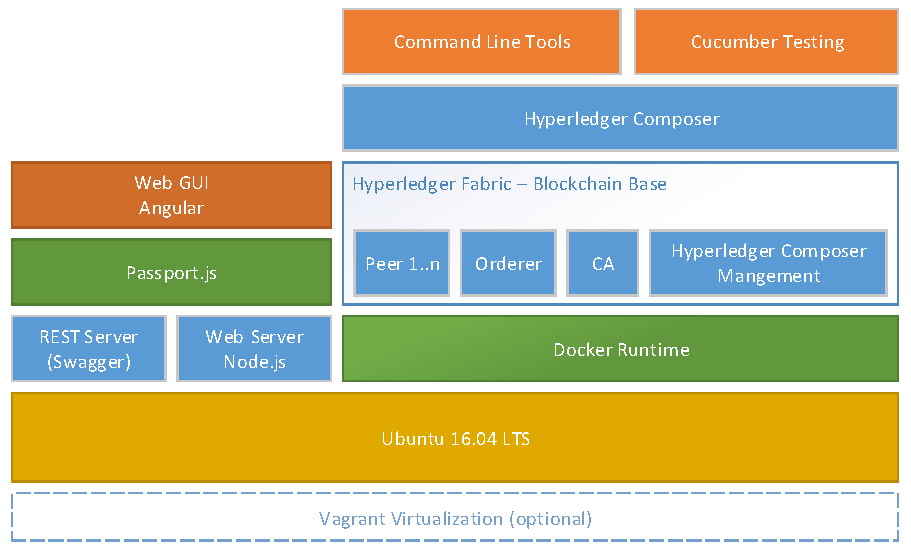
\includegraphics[width=0.7\textwidth, clip, trim=1mm 1mm 1mm 1mm]{Figures/solution-stack}
  \caption{\bf\small Technologies involved for the final solution stack}
  \label{fig:solution-stack}
\end{figure}

As Hyperledger Fabric and Composer are working properly only on MacOs and Linux operating systems there exists an option which includes virtualizsation. On GitHub\footnote{\url{https://github.com/hirsche/hyperledger}} a Vagrant assisted Hyper-V or VirtualBox Machine may be started proving an Ubuntu 16.04 eco-system which is also explained in the next section.